% % \documentclass[manuscript.tex]{subfiles}
% \documentclass[12pt,a4paper]{report} %,openright,twoside
% \usepackage{thesisstyle}
% \addbibresource{bib/PhD.bib}
% \setcounter{chapter}{4}
% \begin{document}

%brings together the key findings and contributions of the research as a whole
% provide a synthesis of the work as a whole presented in the body of the thesis.
% It is important that this final chapter demonstrates the collective contribution to knowledge provided by the research described in the thesis,
% and provide overall conclusions that address the research aims.

\chapter{Future work}
\label{ch:futurework}
The outputs of machine learning models are regarded with apprehension in geophysics practice due to the perceived “black box” of these methods \parencite{delaatAlgorithmicDecisionMakingBased2018,rudinStopExplainingBlack2019}, and the impact these models may have on subsequent interpretation.
As widely accepted by the geoscience community, all models are wrong, but some models are useful, and this extends to machine learning models.

When a domain expert encounters low-resolution grid data, they may observe which gridding method was used, the line spacing and direction, and form their understanding of potential aliasing and spurious anomalies in the grid accordingly.
Assisted by this understanding, they can infer geological features with varying degrees of confidence.
The SR method however does not consider these constraints, because imputation is purely based on features extractable by the model.
This was demonstrated to introduce noise or artefacts during SR inference, as well as the incorrect enhancement of artefacts in low-resolution data such as aliased geological strike.
However, given the uncertainty of geological interpretation of geophysics data \parencite{sivarajahIdentifyingEffectiveInterpretation2013} SR outputs may be used as an auxiliary data when interpreting low-resolution magnetic features.
The domain expert can then use the SR grid to reassure or reassess the original low-resolution grid interpretation and improve their confidence accordingly.

Super-resolution for geophysics is not yet characterised and requires further efforts towards improving reliability before wide-spread adoption in practice.
This section proposes four avenues for future research:
\begin{enumerate}
    \item{} Exploring the impact on geological mapping from the use of SR,
    \item{} Understanding the impact of choices in training super-resolution for domain specific tasks,
    \item{} Identifying an improved image quality assessment for gridded potential field data and,
    \item{} Investigating the use of a physics-informed approach for SR and implicit representation.
\end{enumerate}

\section[Super-resolution impact on geological interpretation]{The impact of super-resolution on geological interpretation}
The super-resolution outputs from the methods presented in this thesis have improved structural accuracy over the low-resolution grids.
This is likely to have a positive impact on the detection of features such as lineaments and unit boundaries for geological interpretation from magnetic data.
However, despite the reduction of introduced structural inaccuracies with the use of open access training data in \Cref{ch:paper2}, it is likely that some features with specific structural geometries will still be incorrectly super-resolved.
A domain expert may be able to recognise structures that are inconsistent using auxiliary information and the regional geological context, but machine processed super-resolution grids will use these data as provided.
In order to improve the adoption of SR for geological interpretation from potential field data, a rigorous study of the impact of SR on interpretation outcomes is required.
This could be a geological mapping task, such as the reinterpretation of regional geology using super-resolution upscaled regional magnetic TMI grids.
Comparison could then be made for the accuracy and benefit of a super-resolution method compared to the existing low-resolution interpretation.
However, such analysis will be difficult to perform with respect to different interpreters' variability in pattern recognition, especially in the context of their confidence in the reliability of the super-resolution product.
Previously, \textcite{sivarajahIdentifyingEffectiveInterpretation2013} reported significant variability between individuals when detecting geological targets from magnetic geophysics data.
A more reliable, repeatable and quantifiable approach would use automated pattern recognition methods developed for geophysical features.
For example, the automated lineament detection technique of \textcite{holdenAutomaticIdentificationResponses2011,holdenAutomatedAnalysisRegional2008} could be applied to low-resolution and SR grids, to compare their delineated features.

\section[Super-resolution for domain specific tasks]{A structured approach to training super-resolution for domain specific tasks}
Several models were implemented throughout \Cref{ch:paper1,ch:paper2}, namely RDN\textdaggerdbl{}, ESRGAN+, and LTE\@.
% However, the most important choice in developing a performant super-resolution neural network for real-world aeromagnetic survey data was the choice of training data.
The work in \Cref{ch:paper1} was prepared for publication prior the release of a large and varied synthetic geology training dataset \parencite{jessellNoddyverseMassiveData2022}.
It was seen in \Cref{ch:paper2} that this data improved model performance for a range of features by using transfer learning for pre-training.
% This transfer learning approach for training data is also found to be useful for RDN\textdaggerdbl{} and ESRGAN\@.
Here, the use of synthetic and real-world line spacing sampled data approach used with LTE in \Cref{ch:paper2} are adopted for the RDN\textdaggerdbl{} and ESRGAN+ models.
\Cref{fig:modcomp} shows RDN\textdaggerdbl{}, ESRGAN+, and LTE predicting accurate structural features when upscaling \qty{320}{\m} data to \qty{80}{\m} line spacing.
While each model has different hyperparameters due to the different architectures in use, the SR prediction converges toward similar structures, with ESRGAN+ containing additional noise.
It can be interpreted that the challenge of super-resolution for this tasks is predominantly a question of providing suitable and sufficient training data, and is less constrained to neural network choices.

\begin{landscape}
    \begin{figure}[hbtp]
        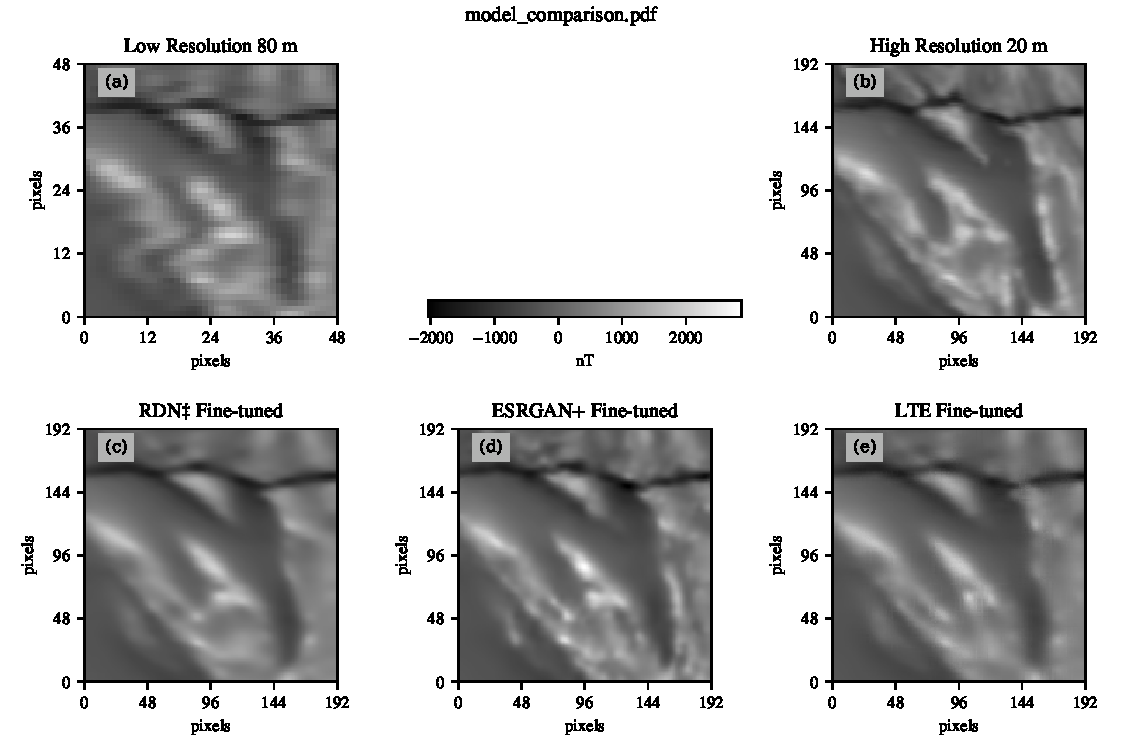
\includegraphics[width=\linewidth,trim={0 0 0 5mm},clip]{fig/etc/model_comparison_v2.pdf}
        \caption[Comparison between the three SR architectures]{
            A comparison between all deep learning super-resolution methods presented in \Cref{ch:paper1} and \Cref{ch:paper2}, using the realistic low-resolution transform developed in \Cref{ch:paper2}.
            a) The low-resolution input, b) The high-resolution target, c) The RDN\textdaggerdbl{} SR prediction, d) The ESRGAN+ SR prediction, and e) The LTE SR prediction.}
        The baseline model for c) and d) was trained for 7 hours on the synthetic dataset described in \Cref{sec:2methods}.
        c) was fine-tuned for 1.5 hours, while d) was fine-tuned for 4.3 hours.
        The training of e) is described in \Cref{sec:finetune}.
        \label{fig:modcomp}
    \end{figure}
\end{landscape}

Given the similar performance between the three distinct architectures, instead of investigating novel SR networks for geophysics super-resolution, an important future work would be understanding the data dependencies of a successful model. For example, filtering the synthetic dataset by event history label to prepare bespoke models for specific geological domains to improve performance at the cost of generalisation.

Magnetic data in different geological contexts are subject to a mixture of statistical distributions \parencite{khokhlovCauseNonGaussianDistribution2017}. Investigation is also required to identify a robust normalisation method accounting for high dynamic range and the structural significance contained in the long tails of the distributions of magnetic intensities.

\section{Image quality assessment for potential field grids}
Model performance is quantified using image quality assessments (IQA) such as peak signal-to-noise ratio (PSNR), structural similarity index (SSIM), feature similarity index (FSIM), or many others.
For supervised tasks, a full reference metric can be calculated between the super-resolution prediction and the high-resolution target.
In the works presented in \Cref{ch:paper1,ch:paper2,ch:paper3}, PSNR and SSIM are used to quantify the performance of the proposed methods in transforming low-resolution grids to high resolution.
However, properties of magnetic grid data are distinct to the images for which these metrics are designed.
%   While SSIM uses structural information present in the Fourier transformed input in combination with local gradient magnitude for value accuracy,
Consistently high SSIM scores are assigned to grids that are perceptually poor matches to the target.
High SSIM values are noted in other geophysical grid investigations which report SSIM metrics \parencite{wangDeeplearningbasedSeismicData2018,bavandsavadkoohiHighresolutionAeromagneticMap2023}.
An investigation to identify a more appropriate IQA for potential field grids is required, which accounts for the distinct nature of these data and better reflects the predicted quality of geological interpretation.
This may be benefit by automated analysis methods as mentioned above.

\section{Geophysics-informed neural networks}
Potential fields are constrained by several well understood physical laws, and gridded data ideally conform to these properties for use in inversion applications and further numerical processing.
Geological interpretation is less reliant on this adherence, however \emph{a priori} information used in physics-informed neural networks improve training speed and model performance \parencite{raissiPhysicsinformedNeuralNetworks2019}, and are especially useful in data-constrained domains such as geophysics.

It is possible to broaden the definition and extend the concept of informed networks to the use of generative adversarial networks in \Cref{ch:paper1}.
In these networks, the informing method is termed discriminator loss, and is performed by a classification network conditioned to identify images as `realistic' or `not realistic', depending on features learned to be important within the target data by the discriminator.
Using crafted or learned criterions to inform a neural network greatly assists with learning high quality models, and either approach may be useful in geophysics to address the paucity of ground truth.
In addition, demonstrating the enforcement of physical properties of potential fields for model outputs may address apprehension for machine learning in geophysics practice.

\printbibliography{}

\chapter{Conclusions}
\label{ch:conclusions}
This thesis presented contemporary methods in deep learning to enhance potential field methods in geoscience.
By including both synthetic and real survey data for training and case studies, it was established that these methods could generalise to real-world applications.

To the best of my knowledge, \Cref{ch:paper1} presents the first investigation in the literature of the super-resolution enhancement of gridded aerogeophysical data.
Prior to this work, it was unknown how well SR methods developed for natural images would adapt to the features and high dynamic range present within magnetic grids, or the challenges faced in developing a training dataset for these data.
We established that the CNN SR methods RDN\textdaggerdbl{} and ESRGAN+ could be trained to upsample low-resolution textures in magnetic grids by a factor of four, and that the results were more accurate than bicubic upsampling in the real-world case study region.
The ESRGAN+ method used in \Cref{ch:paper2} enhanced resolution, however it introduced significant spurious features, masking the enhancement.
Hence, the method based on RDN\textdaggerdbl{} was preferred.
We identified the need for additional representative training data to investigate transferability of the method to other geological domains, and a realistic method to generate low-resolution training data.

The challenge of training data availability was addressed in \Cref{ch:paper2}, where we investigated the use of geologically varied synthetic data to train a baseline model, fine-tuning with real-world data, and simulating realistic line sampling to create low-resolution data.
We implemented the contemporary LTE network to perform this investigation.
Data sampled at four times wider line spacing showed increased structural accuracy when fine-tuned with real-world data.
Additionally, spurious features in the baseline model were correctly resolved when fine-tuned.
We identified opportunities for more detailed investigations using a filtered approach in selecting training data, and these were outlined in \Cref{ch:futurework}.

The contribution in \Cref{ch:paper3} used coordinate multilayer perceptron neural networks to learn a representation of the function that describes a surveyed potential field extent.
To my knowledge, this is the first time implicit neural representation of aerogeophysical survey data has been reported in the literature.
It was seen that these networks are highly suited for processing spatial data such as point sampled geophysics surveys.
The contribution is capable of predicting regularly spaced grids from scattered survey point data, and can be used as a novel method to calculate derivatives of a potential field from the learnt representation, both task which are fundamental to interpretation and processing in geophysics.
By commencing the methods from point sample data, the number of individual processing steps is reduced, and the application is fully trainable.
Continued advances in the recent field of CMLPs will improve the capacity of the method for representing high-resolution aeromagnetic data.

We identify opportunities in \Cref{ch:futurework} for future work stemming from our contribution  of enhancing potential field methods in geophysics.

% \end{document}